\documentclass[aspectratio=169]{beamer}

\mode<presentation> {
\usetheme{SimplePlus} 
\usecolortheme{dolphin}
\setbeamertemplate{navigation symbols}{}
}

\usepackage{graphicx} 
\usepackage{booktabs} 
\usepackage[export]{adjustbox}
\usepackage{blindtext}
\usepackage{hyperref}
\usepackage{graphicx}
\usepackage{amssymb}
\usepackage{amsmath}
\usepackage{bbm}
\usepackage{pgfplots}
\usetikzlibrary{intersections}
\pgfplotsset{compat=1.16}
\usepackage{tikz}
\usetikzlibrary{arrows.meta}
\usepackage[round]{natbib}
\bibliographystyle{apalike}
\usepackage{blindtext}
\usepackage{hyperref}
\usepackage{multirow,array}
\usepackage{threeparttable}
\usepackage[dvipsnames]{xcolor}
\usepackage[T1]{fontenc}\usepackage{lmodern}


\title[Informality and financial frictions]{\Huge \textbf{Informality and financial frictions}} 
\author{David Morales \and Daniela Puggioni}

\author[Morales \& Puggioni]{\textbf{David Morales} \inst{1} \and \textbf{Daniela Puggioni} \inst{2}}
\institute[TSE \and Banxico]{ \inst{1} \textbf{Toulouse School of Economics} \\
david.morales@tse-fr.eu \and 
\inst{2} \textbf{Bank of Mexico}} 

\date[May 28, 2026] 
{\Large \textbf{Macro Workshop}\\
May 28, 2026}

\begin{document}

%------------------------------------------------
\begin{frame}[noframenumbering] 
\titlepage
\end{frame}

%------------------------------------------------

\begin{frame}{Most bank loans goes to the informal sector} 

\textcolor{BrickRed}{\textbf{Informal}}: A firm w/ positive revenue and workers but no Social Security contributions.
\pause

\textbf{Canonical view}: Credit for formal firms (collateral, $\cdots$). Informal are credit-rationed
\begin{itemize}
    \item We should see most entrepreneurial loans going to formal firms.
\end{itemize}
\pause
\begin{center}
    \large In most LMIC, \textbf{the opposite is true}: 
\end{center}

\begin{center}
    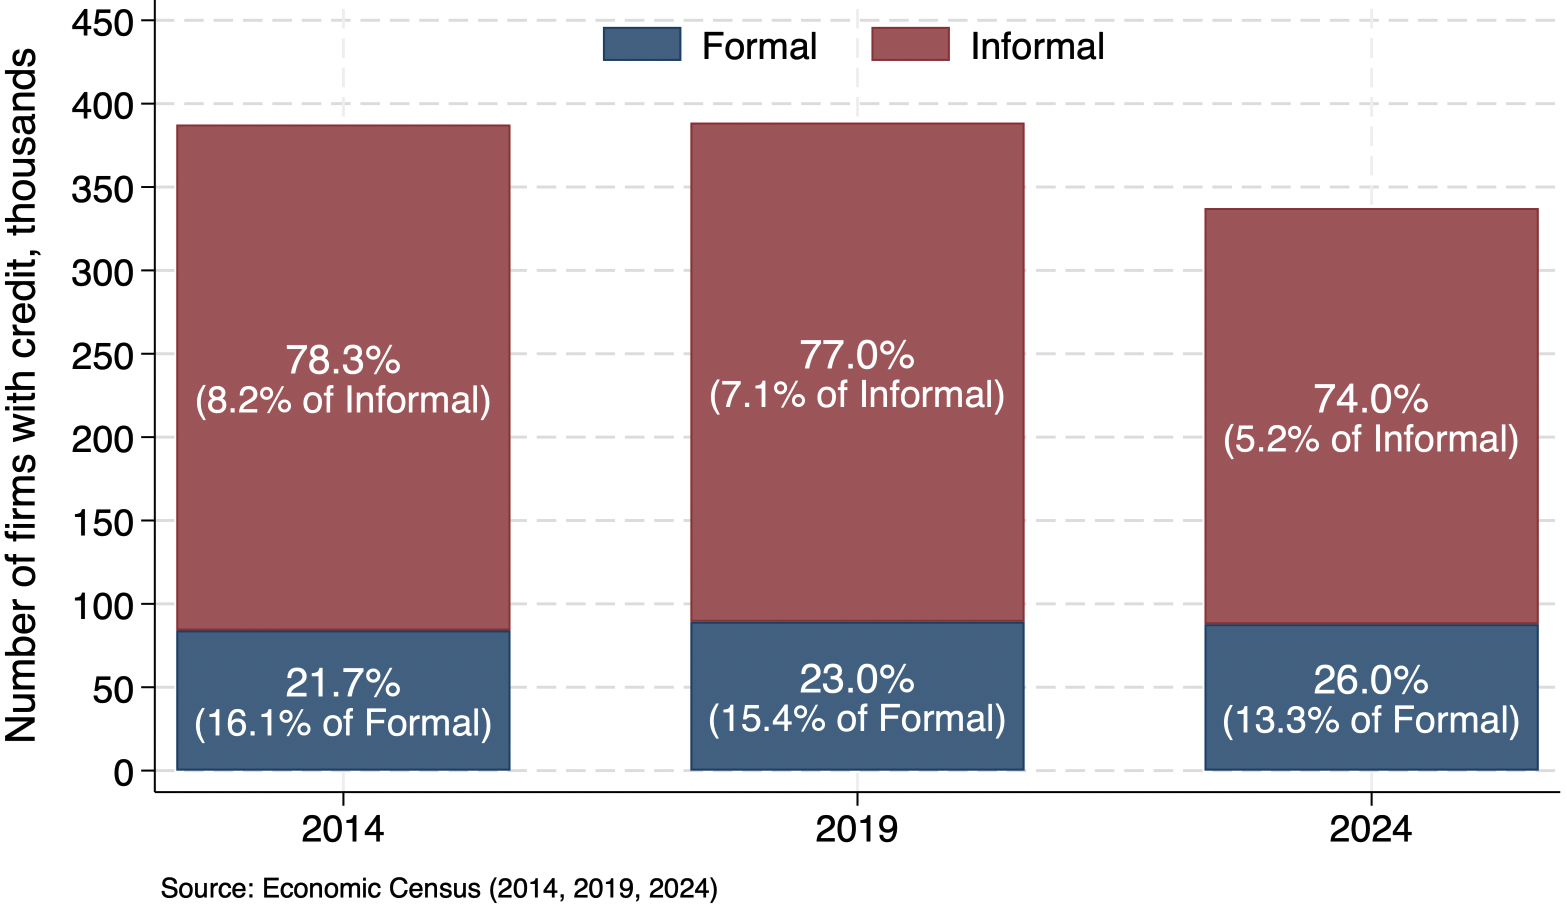
\includegraphics[scale=0.34]{slides_material/firm_dist_g.png}
\end{center}

\end{frame}

%------------------------------------------------

\begin{frame}{There is substantial firm dynamics}

\textbf{Canonical view}: Segmented Formal-Informal sectors \textcolor{lightgray}{\cite{la2014informality}}.
\begin{itemize}
    \item We expect to see limited dynamics and Formal-Informal transitions.
\end{itemize}

\pause

\begin{center}
    \large Again, in most LMIC, \textbf{the opposite is true}: 
\end{center}

\begin{center}
    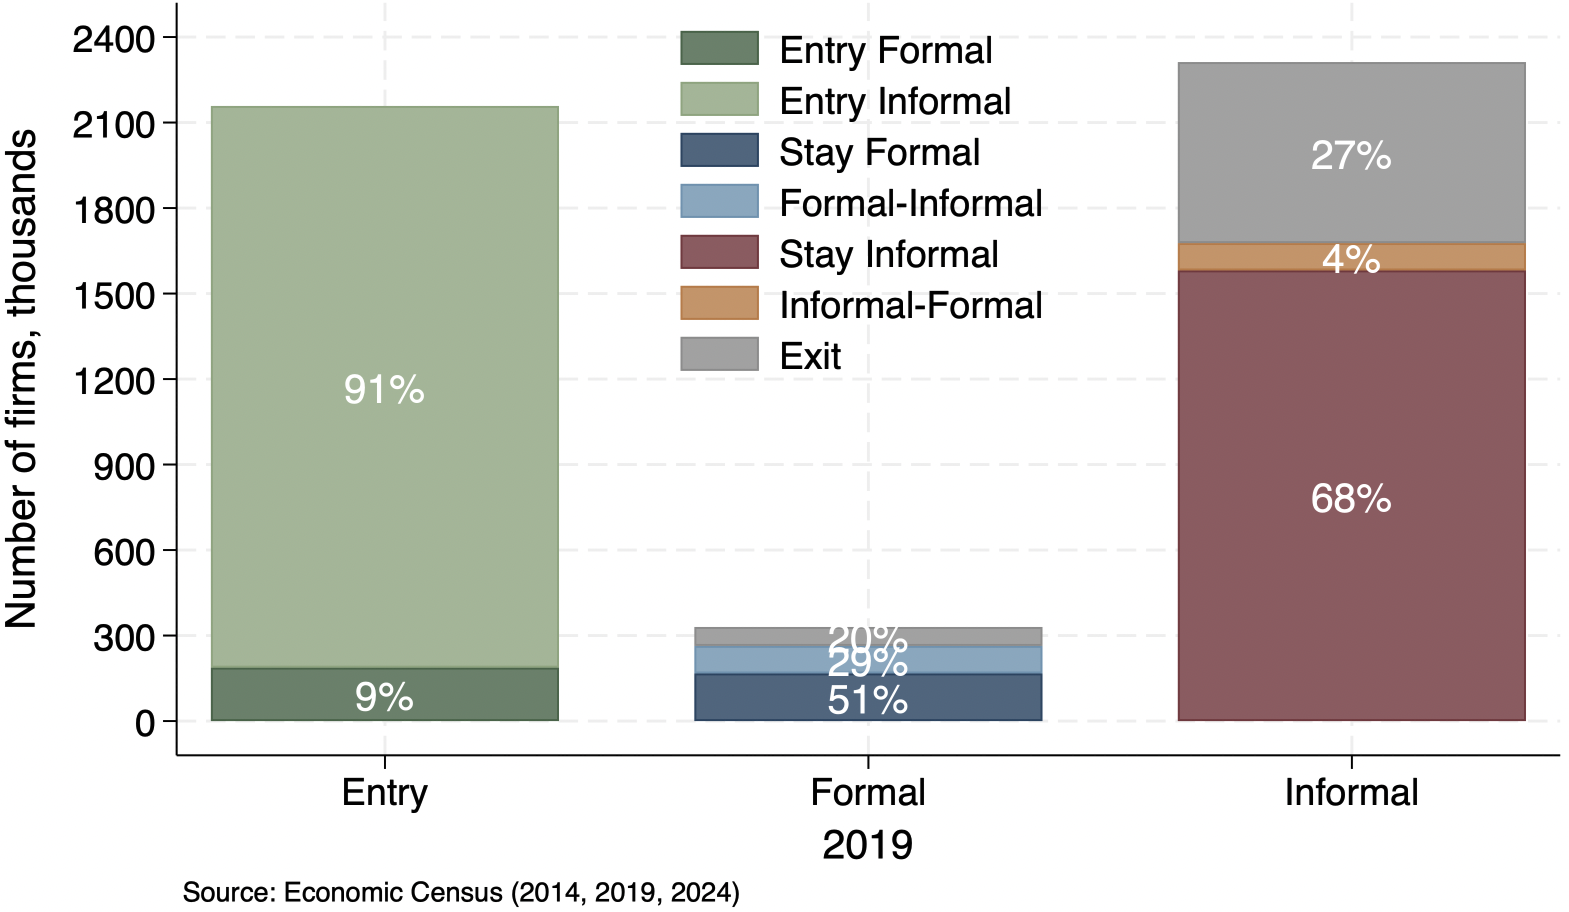
\includegraphics[scale=0.35]{slides_material/transition_g.png}
\end{center}

\end{frame}

%------------------------------------------------


\begin{frame}{This paper}

\begin{center}
    \Large \textbf{RQ}: Can bank loans explain firm dynamics?
\end{center}

\vspace{4mm}
\pause

\textbf{Answer}
\begin{itemize}
    \item Credit increases entrepreneurial activity, but (surprisingly) mainly in informal sector.
\end{itemize}

\vspace{5mm}
\pause

\textbf{Method}
\begin{itemize}
    \item Shift-share IV with exogenous shift.
    \item Dynamic model of firm transitions w/financial constraints.
\end{itemize}

\vspace{5mm}
\pause

\textbf{Why it matters}
\begin{itemize}
    \item Financial development can increase firm activity and informality.
\end{itemize}

\vspace{5mm}
\pause

\textbf{Contribution}
\begin{itemize}
    \item Document novel firm dynamics and causal evidence.
\end{itemize}

\end{frame}

%------------------------------------------------

\begin{frame}{Literature}

Financial access effects on firm activity \textcolor{lightgray}{\citep{amiti2018much,greenstone2020credit,gutierrez2023credit,khwaja2008tracing,chodorow2014employment}, etc.}
 \begin{itemize}
    \item \textbf{Literature takeaway}: Credit increases employment, productivity, and formalization.
    \item \textbf{Contribution}: Evidence on credits increasing informality.
 \end{itemize}

\vspace{10mm}

Informality causes and consequences \textcolor{lightgray}{\citep{ulyssea2018firms,meghir2015wages,la2014informality,almeida2012enforcement,busso2012formal,adom2025structural}, etc.}
\begin{itemize}
    \item \textbf{Literature takeaway}: Little firm dynamics and formal status as absorbing state.
     \item \textbf{Contribution}: Novel firm dynamics, w/formal firms possibly moving into informality.
 \end{itemize}

\vspace{10mm}

\begin{itemize}
    \item[$\Rightarrow$] \Large \textbf{This paper}: Link of formality decisions and credit access. 
\end{itemize}



\end{frame}

%------------------------------------------------

\begin{frame}[noframenumbering]{Outline}

\Large

1) Data

\vspace{5mm}

\textcolor{lightgray}{2) Empirical Strategy}

\vspace{5mm}

\textcolor{lightgray}{3) Results}

\vspace{5mm}

\textcolor{lightgray}{4) Model}

\vspace{5mm}

\textcolor{lightgray}{5) Counterfactual}

\vspace{5mm}

\textcolor{lightgray}{6) Conclusions}


\end{frame}

% %------------------------------------------------


\begin{frame}{Data}

\textbf{Mexican data}

\vspace{5mm}

\begin{itemize}
    \item Matched bank-employer-employee data \textcolor{gray}{Social Security (IMSS) +  Exchange \& Security Commission (CNBV)}
    \begin{itemize}
        \item 20 years of monthly data.
        \item Universe of formal workers.
        \item Banking loans to formal and informal firms.
    \end{itemize}
    \vspace{5mm}
    \item Economic Census \textcolor{gray}{(EC)}
    \begin{itemize}
        \item Every 5 years (2009, 2014, 2019, \& 2024).
        \item Formal and informal firm level data used for the firm 5-years transitions.
    \end{itemize}
    \vspace{5mm}
    \item Data: 703 markets = commuting zones, 89 banks, and $\approx$ 4.5 million firms.
\end{itemize}

\vspace{5mm}

\begin{center}
    \large \textbf{Key feature:} Observe credit + firm dynamics + economic outcomes.
\end{center}
\end{frame}

%------------------------------------------------

\begin{frame}[noframenumbering]{Outline}

\Large

\textcolor{lightgray}{1) Data}

\vspace{5mm}

2) Empirical Strategy

\vspace{5mm}

\textcolor{lightgray}{3) Results}

\vspace{5mm}

\textcolor{lightgray}{4) Model}

\vspace{5mm}

\textcolor{lightgray}{5) Counterfactual}

\vspace{5mm}

\textcolor{lightgray}{6) Conclusions}

\end{frame}

%------------------------------------------------


\begin{frame}{Identification: Exploit cross-market exposure to bank shocks} 

\textbf{Identification challenge}: Credit is endogenous (demand shocks, reverse causality).
\begin{itemize}
    \item[$\Rightarrow$] \textbf{Solution} Shift-Share IV instrument with exogenous shift \textcolor{lightgray}{\citep{borusyak2022quasi}}. 
\end{itemize}

\vspace{5mm}
\pause

\textbf{Identification:} Compare markets exposed to different bank national credit changes.

\vspace{5mm}


\textbf{Identifying assumption}: Outcome $\perp$ shift (bank FE), only affected through loans.

\vspace{5mm}
\pause

\textbf{Violation of the assumption} if for example
\begin{itemize}
    \item In an oil boom, a bank specializing on oil-sector increases loans, and simultaneously a oil-dependent market increases firm growth due to non-credit reasons. 
    \item[$\Rightarrow$] \textbf{Solution}: Control for state-year FE and robustness checks.
\end{itemize}

\end{frame}

%------------------------------------------------

\begin{frame}{\textbf{Empirical strategy}} \label{iv_market_level}

\textbf{Intuition}: Mkt credit grows due to 1) local firms want to borrow (demand) and 2) banks operating locally grow nationally (supply) $\Rightarrow$ We isolate supply and ask: where did it go?

\vspace{5mm}
\pause

\textbf{1) Decompose demand-supply}: Regress bank-market credit on bank and market FE:

\begin{equation*}
    \Delta \ln(C_{m,b,t}) = \alpha_{m,t} + \gamma_{b,t} + \epsilon_{m,b,t}, \quad \Rightarrow \quad \hat{\gamma}_{b,t} = \text{Exogenous shift.} 
\end{equation*}
\pause

\textbf{2) Share}: Banks' share of total loans in a market in previous period:

\begin{equation*}
    s_{b,m,t-1} = \frac{L_{b,m,t-1}}{\sum_b L_{b,m,t-1}}, \quad \Rightarrow \quad s_{b,m,t-1} = \text{Identifying variation.} 
\end{equation*}
\pause

\textbf{3) Instrument}: Bank change in credit supply weighted by market share.  \hyperlink{iv_bank_level}{\beamergotobutton{Shock}} \hyperlink{loo}{\beamergotobutton{LOO}}

\begin{equation*}
    \hat{Z}_{m,t} = \sum_b \left( s_{b,m,t-1} \times \hat{\gamma}_{b,t} \right) 
\end{equation*}

% \begin{center}
%     \Large \textbf{Interpretation}: Different exposure of markets to exogenous bank shocks.
% \end{center}

\end{frame}

%------------------------------------------------

\begin{frame}[noframenumbering]{Outline}

\Large

\textcolor{lightgray}{1) Data}

\vspace{5mm}

\textcolor{lightgray}{2) Empirical Strategy}

\vspace{5mm}

3) Results

\vspace{5mm}

\textcolor{lightgray}{4) Model}

\vspace{5mm}

\textcolor{lightgray}{5) Counterfactual}

\vspace{5mm}

\textcolor{lightgray}{6) Conclusions}

\end{frame}

%------------------------------------------------

\begin{frame}{The instrument is relevant}

\begin{center}
    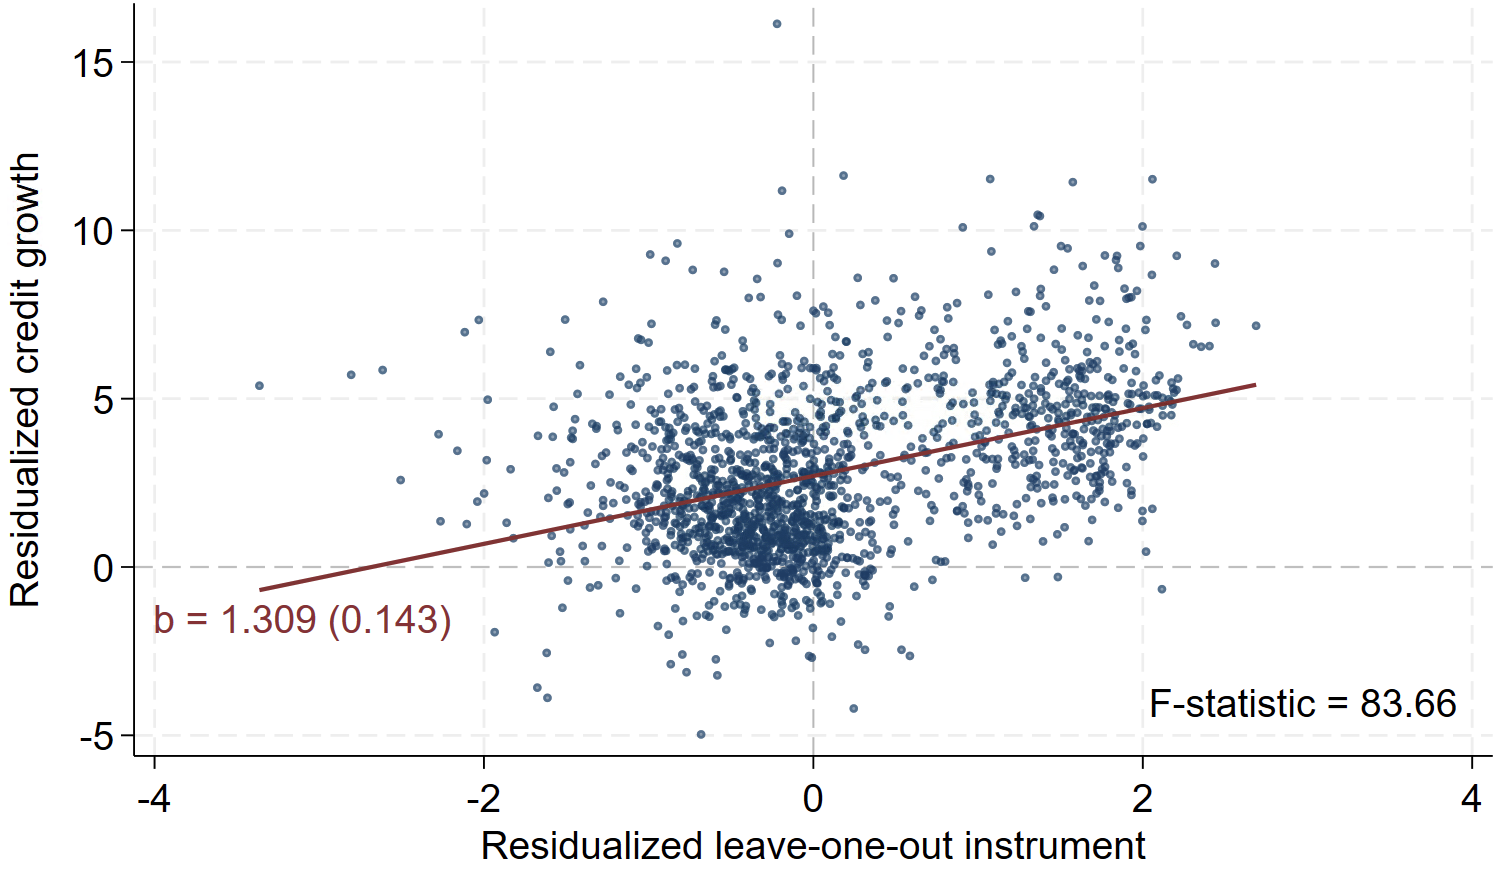
\includegraphics[scale=0.20]{slides_material/first_stage.png}
\end{center}

\begin{itemize}
    \item Relevant instrument: First stage F-stat = 23 
    \item Effective N varies across years; results are robust to dropping concentrated markets 
\end{itemize}

\begin{center}
    \Large \textbf{Interpretation}: Bank shocks capture supply variation.
\end{center}

\end{frame}

%------------------------------------------------

\begin{frame}{Credit expansion increases firm activity,  mostly informally} \label{main_result}

\begin{itemize}
    \item[$\Rightarrow$] $\uparrow$ 1\% in credit yields + 23 firms, + 24 more informal and - 1  formal, on avg market.
\end{itemize}
\begin{center}
    \begin{tabular}{lccc}
    \toprule
    \multicolumn{4}{c}{\textbf{Dependent variable}: Log Nb. of firms} \\
    \cmidrule(lr){2-4}
              & Total & Formal & Informal \\
    \midrule
    Log loans &  0.328  & -0.085  & 0.401 \\
              & (0.049) & (0.015) & (0.059) \\
    \midrule
    Mean (level) & 7,152 & 868 & 6,284 \\
    \bottomrule
    \end{tabular}
\end{center}

\vspace{5mm}
\pause

\begin{center}
    \large However, $\cdots$ is it due to the entry, exit, or transition?
\end{center}

\vspace{10mm}

\begin{center}
    \textbf{Robustness}: \quad \hyperlink{ols}{\beamergotobutton{OLS}} \quad \hyperlink{unconcentrated}{\beamergotobutton{Non-concentrated markets}} \quad \hyperlink{llm_level}{\beamergotobutton{Market level}} \quad  \hyperlink{balance}{\beamergotobutton{Balance test}} \quad \hyperlink{placebo}{\beamergotobutton{Placebo test}}
\end{center}

\end{frame}

%------------------------------------------------

\begin{frame}{Mechanism decomposition: Informal entry dominates}

\begin{columns}[T] 
    \begin{column}{0.6\textwidth} 
        \begin{center}
        \vspace{-5mm}
            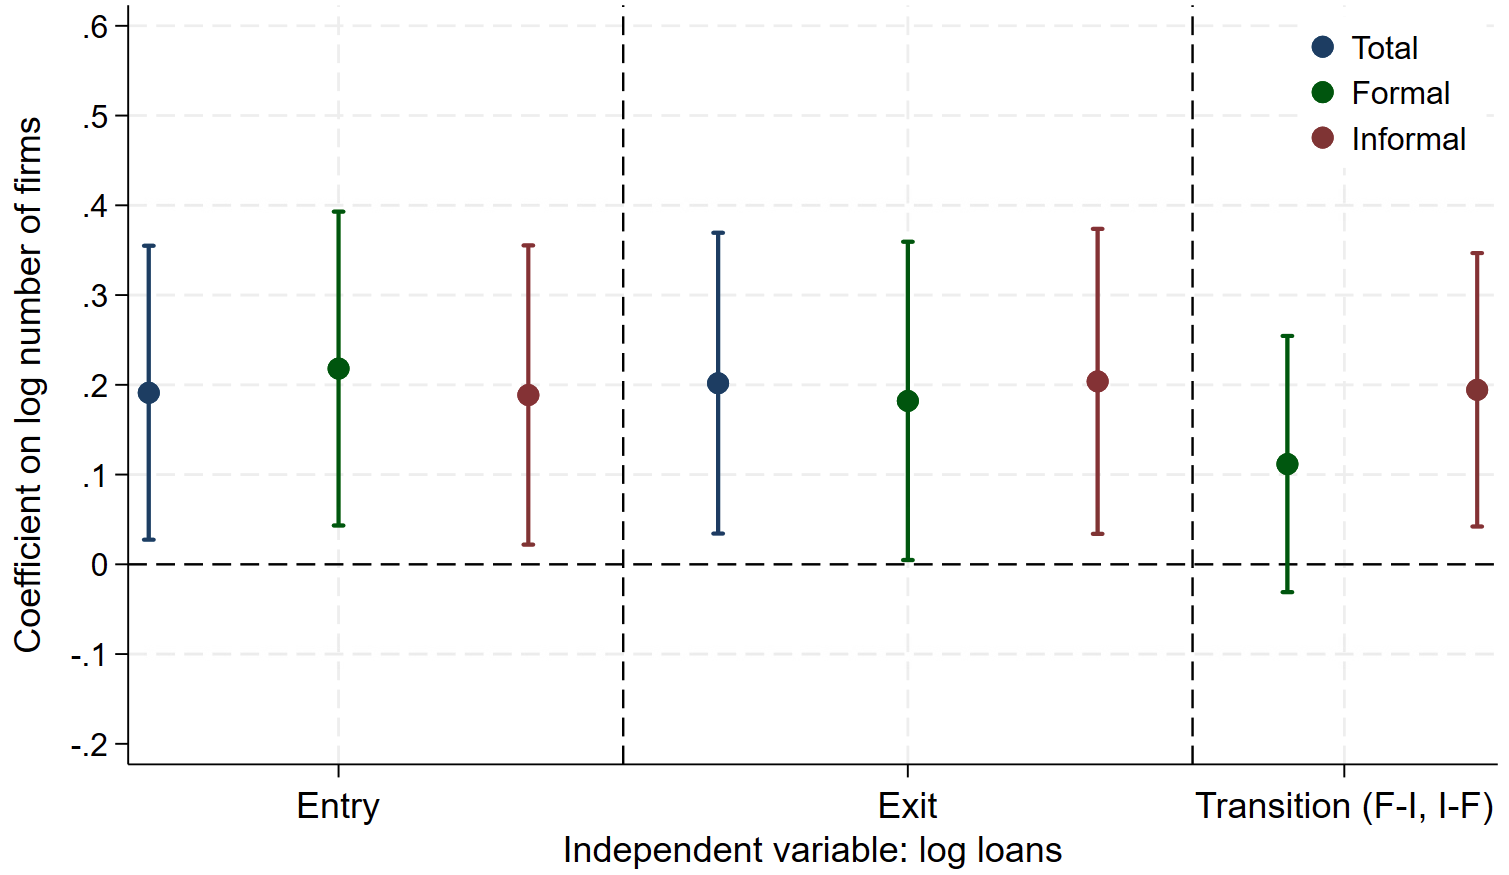
\includegraphics[scale=0.2]{slides_material/decomp.png}
        \end{center}
    \end{column}

    \begin{column}{0.4\textwidth} 
        \begin{itemize}
            \vspace{5mm}
            \item $\uparrow$ 1\% in credit yields
            \begin{itemize}
                \item +8 entering firms.
                \begin{itemize}
                    \item +9 informal.
                    \item -1 formal.
                \end{itemize}
                \item +5 exiting informal firms.
                \begin{itemize}
                    \item + Competition.
                \end{itemize}
                \item -1 formal-informal.
            \end{itemize}
        \end{itemize}
        \vspace{5mm}
        \pause
        \textbf{Significant 5-year start-up rate}:
        
        + 0.11 p.p. v.s. - 0.78 in USA \textcolor{gray}{\cite{pugsley2019grown}}.
    \end{column}
\end{columns}

\end{frame}

%------------------------------------------------
\begin{frame}{Most credit adjustments goes to informal firms}

\large \textbf{Q}: What firms are more affected by the change in credit?

\vspace{5mm}

\begin{center}
    \begin{tabular}{lccc}
    \toprule
    \multicolumn{4}{c}{\textbf{Dependent variable}: Log Nb. of firms w/ credit} \\
    \cmidrule(lr){2-4}
              & Total & Formal & Informal \\
    \midrule
    Log loans &  0.152  & -0.051  & 0.274 \\
              & (0.023) & (0.019) & (0.037) \\
    \midrule
    Mean (level) & 454 & 344 & 110 \\
    \bottomrule
    \end{tabular}
\end{center}

\vspace{5mm}

\begin{center}
    \large \textbf{A}: When banks adjust credit, their main adjusting margin is on informal firms.
\end{center}

\end{frame}

%------------------------------------------------


\begin{frame}{+ informal workers, - avg productivity, \& + total productivity}

\begin{center}
    \begin{tabular}{lcccccc}
    \toprule
     & \multicolumn{3}{c}{Log nb. workes} & \multicolumn{2}{c}{Log average} & \multirow{2}{*}{Log total VA} \\
    \cmidrule(lr){2-4} \cmidrule(lr){5-6}
     & Total & Formal & Informal & Formal wage & VA &  \\
    \midrule
    Log loans 
    & 0.123 & -0.034 & 0.157 & 0.022  & -0.239  & 0.088 \\
    & (0.030) & (0.018) & (0.019) & (0.003) & (0.042) & (0.018) \\
    \midrule
    Mean (level) & 19,521 & 5,566 & 13,955 & 10.9 & 48.8 & 0.9 m. \\
    \bottomrule
\end{tabular}
\begin{tablenotes}[flushleft]
\tiny
\item Notes: The annual average added value, and the annual total value added in a market are 174 MXN, 780 MXN, and 14.5 million MXN, respectively, which using an exchange rate of 16 MXN per USD are equivalent to 10.9 USD, 48.8 USD, and 0.9 million USD, respectively.
\end{tablenotes}
\end{center}
\pause

\textbf{Bigger effect on worker informality than tax cuts}  \textcolor{gray}{\cite{bobba2021labor,rocha2018lower,campos2020effects}}.

\vspace{5mm}

How to determine mechanisms (tax, constraints, productivity) and its importance? $\cdots$ 

\begin{center}
    \Large \textbf{Model}
\end{center}


\end{frame}

%------------------------------------------------

\begin{frame}[noframenumbering]{Outline}

\Large

\textcolor{lightgray}{1) Data}

\vspace{5mm}

\textcolor{lightgray}{2) Empirical Strategy}

\vspace{5mm}

\textcolor{lightgray}{3) Results}

\vspace{5mm}

4) Model

\vspace{5mm}

\textcolor{lightgray}{5) Counterfactual}

\vspace{5mm}

\textcolor{lightgray}{6) Conclusions}

\end{frame}

%------------------------------------------------

\begin{frame}{The model must explain the increase on informal firm activity}

\textbf{The model must replicate}

\begin{enumerate}
    \item Credit increases informal entry.
    \item Credit lowers average productivity.
    \item Formalization does not rise mechanically with credit.
\end{enumerate}

\vspace{6mm}

\large
\textbf{Main idea:} More financial access allows low-productivity firms to enter informally.

\end{frame}

%------------------------------------------------

\begin{frame}
\frametitle{Settings}


\textbf{Firms}: Heterogeneous in productivity $\theta \in [\underline{\theta}, \bar{\theta}]$. 

\vspace{5mm}
\pause

\textbf{Technology}: $f(l,k; \theta) = \theta q(l,k)$, well behaved and $q(\cdot)$ w/ decreasing returns to scale. 

\vspace{5mm}
\pause

\textbf{Partial Equilibrium}: We treat wage w as exogenous.

\vspace{5mm}
\pause

\textbf{Mkt structure}: For. \& inf. produce same good, same prices \textcolor{lightgray}{\citep{imbert2023rural}}.


\vspace{5mm}
\pause
    
\textbf{Investment function}: $i(k',k) = k' - (1 - \delta) k$.

\begin{itemize}
    \item \textcolor{gray}{\textbf{Financing cost function}: $\phi_s(k,k',\theta;w) = \phi_s(i(k, k') - \Pi(k,\theta;w)), \quad \forall s \in \{i,f\}$.}
\end{itemize}

\vspace{5mm}
\pause


\textbf{Informal}: $\Pi_i(k,\theta;w) = \max \limits_{\{l\}} \{ \theta q(l,k) - \tau_i(l) w - \bar{c}_i \}$, $\tau_i(l)$ inf. cost \textcolor{lightgray}{\citep{ulyssea2018firms}}.

\vspace{5mm}
\pause

\textbf{Formal profits}: $\Pi_f(k,\theta;w) = \max \limits_{\{l\}} \{ (1 - \tau_y) \theta q(l,k) - (1 + \tau_l) w - \bar{c}_f \}$.

\end{frame}

%------------------------------------------------

\begin{frame}
\frametitle{Timing}

\begin{figure}[h!] 
    \begin{center}
        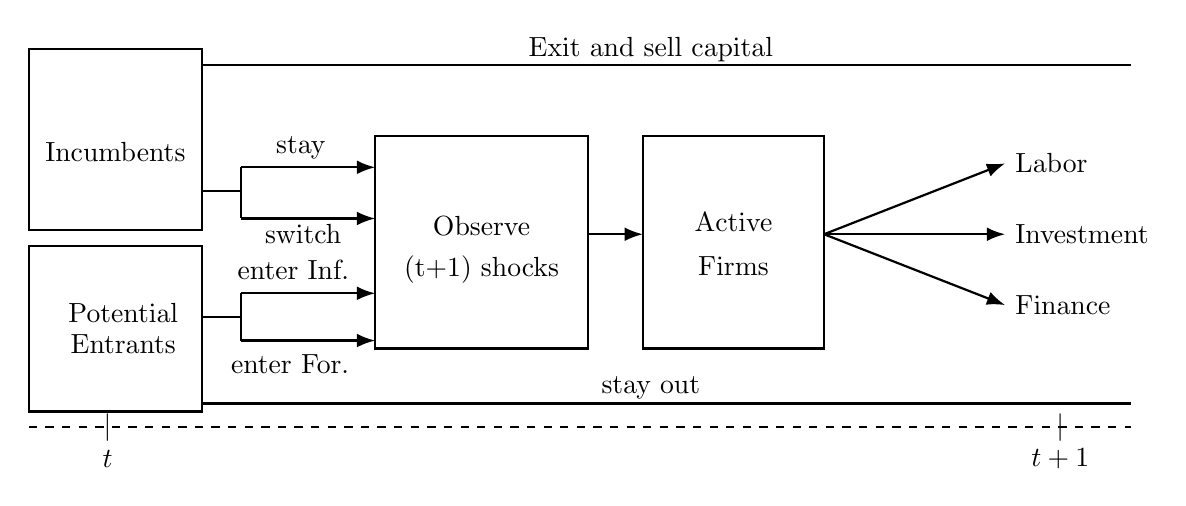
\begin{tikzpicture}[>=Latex, thick]


% timeline
\draw[dashed] (0,0) -- (14,0);
\node at (1.0,0.0) {$|$};
\node at (1.0,-0.4) {$t$};
\node at (13.1,0.0) {$|$};
\node at (13.1,-0.4) {$t+1$};

% title
\node at (7.9,4.8) {Exit and sell capital};
\draw (2.2,4.6) -- (14,4.6);

% left boxes
\draw (0,2.5) rectangle (2.2,4.8);
\node at (1.1,3.5) {Incumbents};

\draw (0,0.2) rectangle (2.2,2.3);
\node at (1.2,1.45) {Potential};
\node at (1.2,1.05) {Entrants};

% observe shocks box
\draw (4.4,1) rectangle (7.1,3.7);
\node at (5.75,2.55) {Observe};
\node at (5.75,2.0) {(t+1) shocks};

% labels on left
\node[left] at (3.9,3.55) {stay};
\node[left] at (4.1,2.45) {switch};
\node[left] at (4.2,2.00) {enter Inf.};
\node[left] at (4.2,0.80) {enter For.};

% three clean arrows into box
\draw[-] (2.2,3.00) -- (2.7,3.00);
\draw[-] (2.7,3.30) -- (2.7,2.65);
\draw[->] (2.7,3.30) -- (4.4,3.30);
\draw[->] (2.7,2.65) -- (4.4,2.65);

\draw[-] (2.2,1.40) -- (2.7,1.40);
\draw[-] (2.7,1.10) -- (2.7,1.70);
\draw[->] (2.7,1.10) -- (4.4,1.10);
\draw[->] (2.7,1.70) -- (4.4,1.70);

% process labels
% \node at (5.8,3.95) {$\ln(\theta_{jt})$};
% \node at (5.8,0.7) {$\ln(\theta_{j1})$};

% stay out dashed line
\draw (2.2,0.3) -- (14,0.3);
\node at (7.9,0.5) {stay out};

% active firms box
\draw (7.8,1) rectangle (10.1,3.7);
\node at (8.95,2.60) {Active};
\node at (8.95,2.05) {Firms};

% arrow observe -> active
\draw[->] (7.1,2.45) -- (7.8,2.45);

% outputs
\draw[->] (10.1,2.45) -- (12.4,3.35);
\draw[->] (10.1,2.45) -- (12.4,2.45);
\draw[->] (10.1,2.45) -- (12.4,1.55);

\node[right] at (12.4,3.35) {Labor};
\node[right] at (12.4,2.45) {Investment};
\node[right] at (12.4,1.55) {Finance};

\end{tikzpicture}
    \end{center}
\end{figure}

\end{frame}

%------------------------------------------------


\begin{frame} \label{back3}
\frametitle{Value functions}

\begin{center}
    \large \textbf{Informal}
\end{center}

\vspace{-10mm}

\begin{multline*}
    V_i(k, \theta; w) = \max\limits_{k'} \{ \overbrace{ \Pi_i(k,\theta;w) - i(k,k') - \phi_i(k,k',\theta;w)}^{\text{Dividends}} + \\
    \beta \max \{ \underbrace{(1 - \delta) k}_{\text{Exit}} , \underbrace{\mathbb{E}[V_i(k',\theta',w) \vert \theta] }_{{\text{Stay Informal}}} , \underbrace{\mathbb{E}[V_f(k',\theta',w) \vert \theta] - c_{if}}_{\text{Transition Informal-Formal}} \} \}
\end{multline*}

\vspace{5mm}

\begin{center}
    \large \textbf{Formal}
\end{center}

\vspace{-10mm}

\begin{multline*}
    V_f(k, \theta; w) = \max\limits_{k'} \{ \overbrace{ \Pi_f(k,\theta;w) - i(k,k') - \phi_f(k,k',\theta;w)}^{\text{Dividends}} + \\ 
    \beta \max \{ \underbrace{(1 - \delta) k}_{\text{Exit}} , \underbrace{\mathbb{E}[V_f(k',\theta',w) \vert \theta]}_{{\text{Stay Formal}}} , \underbrace{\mathbb{E}[V_i(k',\theta',w) \vert \theta] - c_{fi}}_{\text{Transition Formal-Informal}} \} \}
\end{multline*}

\end{frame}

%------------------------------------------------

\begin{frame}
\frametitle{Decision rules} \label{transition}

% \textbf{Capital}: $k'_s(k,\theta;w) = \min \{ arg\max\limits_{k'} \{ V_s(k,\theta;w) \}\}$, k' that does not requires borrowing.

\textbf{Transition}: \hyperlink{threshold}{\beamergotobutton{Unique threshold values}}
\begin{itemize}
    \item \textbf{Inactive}: $t_n(k,\theta;w) = \begin{cases}
        n \text{ if } \theta_i^e  > \theta \text{ (stay inactive)} \\
        i \text{ if } \theta_i^e \leq \theta < \theta_f^e \text{ (enter informal)} \\
        f \text{ if } \theta  \geq \theta_f^e \text{ (enter formal)}
    \end{cases}$
    \item \textbf{Informal}: $t_i(k,\theta;w) = \begin{cases}
        n \text{ if } \theta_i^x  > \theta \text{ (exit as informal)} \\
        i \text{ if } \theta_i^x \leq \theta < \theta_{if} \text{ (stay informal)} \\
        f \text{ if } \theta  \geq \theta_{if} \text{ (transition informal-formal)}
    \end{cases}$
    \item \textbf{Formal}: $t_f(k,\theta;w) = \begin{cases}
        n \text{ if } \theta_f^x  > \theta \text{ (exit as formal)} \\
        i \text{ if } \theta_f^x \leq \theta < \theta_{fi} \text{ (transition formal-informal)} \\
        f \text{ if } \theta  \geq \theta_{fi} \text{ (stay formal)}
    \end{cases}$
\end{itemize}

\end{frame}

%------------------------------------------------

\begin{frame}
\frametitle{Formal and informal unique threshold values}

\begin{center}
    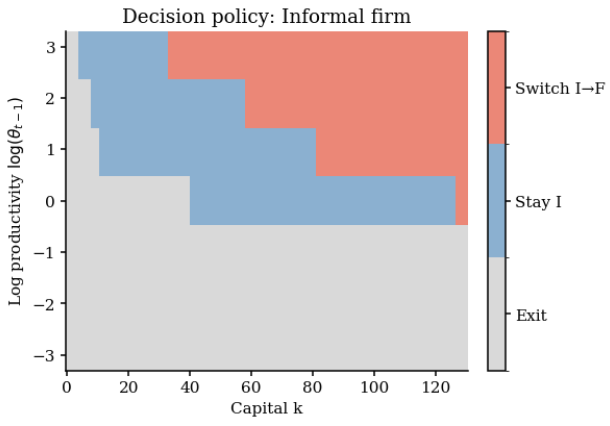
\includegraphics[scale=0.66]{transition_informal.png}
    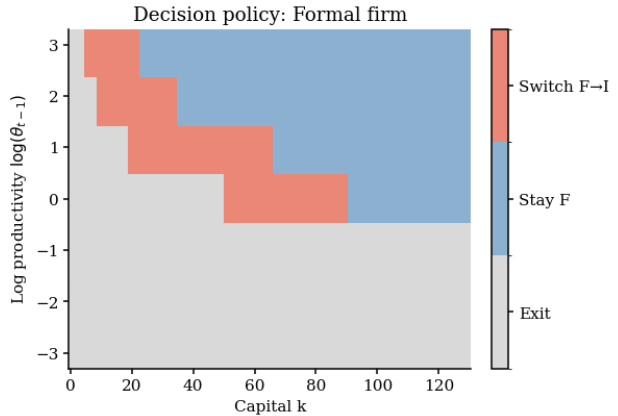
\includegraphics[scale=0.66]{transition_formal.png}
\end{center}

\end{frame}

%------------------------------------------------


\begin{frame}
\frametitle{Inactive unique threshold values}

\begin{center}
    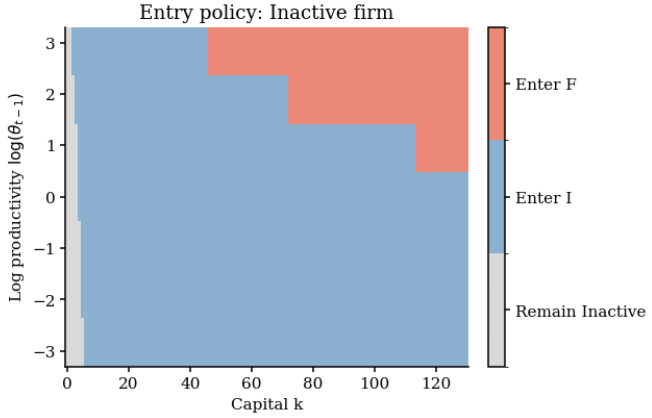
\includegraphics[scale=0.66]{transition_inactive.png}
\end{center}

\end{frame}

%------------------------------------------------

\begin{frame}
\frametitle{\textbf{Model estimation}: SMM} \label{model_estimation}

\textbf{11 Parameters to estimate through SMM}: 
\begin{center}
    $\Theta = \{\rho_i, \rho_f, \mu_{k0}, \sigma_{k0}, c_{ei}, c_{ef}, \phi_{1i}, \phi_{1f}, c_{if}, c_{fi}, c_{f}\}$
\end{center}

\vspace{5mm}

\textbf{Estimation procedure}

\begin{enumerate}
    \item Estimate $\rho_{i}$ and $\rho_{f}$ with 6 moments.
    \item Estimate $\mu_{k0}$, $\sigma_{k0}$, $c_{ei}$, and $c_{ef}$ with 8 moments.
    \item Estimate $\phi_{1i}$, $\phi_{1f}$, $c_{if}$, $c_{fi}$, and $c_f$ with 13 moments.
    \item Joint SMM refinement over all 11 parameters with 27 moments.
\end{enumerate}

\vspace{5mm}

\textbf{Objective function to minimize}:

\begin{center}
    $Q(\Theta) = (m^{model}(\Theta) - m^{data})' W (m^{model}(\Theta) - m^{data})$.
\end{center}

\end{frame}

%------------------------------------------------

\begin{frame}
\frametitle{\textbf{Model estimation}: Parameters to estimate I} \label{parameters1}

\footnotesize
\begin{tabular}{lll}
\hline\hline
\textbf{Parameter} & \textbf{Description} & \textbf{Identification} \\
\hline

\multicolumn{3}{l}{\textit{Technology}} \\
$\alpha$ & Capital elasticity & Production function regression \\
$\nu$    & Labor elasticity   & Production function regression \\
$w$      & Wage               & Normalized to 1 \\
\addlinespace

\multicolumn{3}{l}{\textit{Taxes and Informality Costs}} \\
$\tau_l$ & Payroll tax & Tax policy \\
$\tau_y$ & VAT tax     & Tax policy \\
$\rho_i$ & Informal hiring cost (informal firms) & Moments: $K/L$, employment (informal) \\
$\rho_f$ & Informal hiring cost (formal firms)   & Moments: $K/L$, employment (formal) \\
\addlinespace

\multicolumn{3}{l}{\textit{Productivity Process}} \\
$\rho_u$   & Persistence & AR(1) on residual productivity \\
$\sigma_u$ & Variance    & Std. dev. of AR(1) residuals \\
\addlinespace

\multicolumn{3}{l}{\textit{Capital Accumulation}} \\
$\delta$ & Depreciation rate & Standard value \\
$\beta$  & Discount factor   & $1/(1+r)$ \\
\hline\hline
\end{tabular}

\end{frame}

%------------------------------------------------

\begin{frame}
\frametitle{\textbf{Model estimation}: Parameters to estimate II} \label{parameters2}

\begin{center}
    \footnotesize
    \begin{tabular}{lll}
\hline\hline
\textbf{Parameter} & \textbf{Description} & \textbf{Identification} \\
\hline

\multicolumn{3}{l}{\textit{Financial Constraints}} \\
$\phi_{1i}$ & Cost of funds (informal) & Moments: borrowing, funds, investment (informal) \\
$\phi_{1f}$ & Cost of funds (formal)   & Moments: borrowing, funds, investment (formal) \\
\addlinespace

\multicolumn{3}{l}{\textit{Entry, Exit, and Transitions}} \\
$c_{fi}$ & Formal $\rightarrow$ informal cost & Switching hazard \\
$c_{if}$ & Informal $\rightarrow$ formal cost & Switching hazard \\
$c_{ef}$ & Formal entry cost & Formal entry share \\
$c_{ei}$ & Informal entry cost & Informal entry share \\
$c_f$    & Formal operating cost & Formal share, exit, profits \\
$c_i$    & Informal operating cost & Normalized to 0 \\
\addlinespace

\multicolumn{3}{l}{\textit{Entry Capital}} \\
$\mu_{k0}$    & Mean entrant capital & Moments: capital (age 0--2), $K/L$ \\
$\sigma_{k0}$ & Std. dev. entrant capital & Moments: dispersion, P90 capital \\
\hline\hline
\end{tabular}
\end{center}

\end{frame}

%------------------------------------------------

\begin{frame}[noframenumbering]{Outline}

\Large

\textcolor{lightgray}{1) Data}

\vspace{5mm}

\textcolor{lightgray}{2) Empirical Strategy}

\vspace{5mm}

\textcolor{lightgray}{3) Results}

\vspace{5mm}

\textcolor{lightgray}{4) Model}

\vspace{5mm}

5) Counterfactual

\vspace{5mm}

\textcolor{lightgray}{6) Conclusions}

\end{frame}

%------------------------------------------------

\begin{frame}
\frametitle{\textbf{Counterfactual}: -25\% on informal financial constraints}

\begin{center}
    \textbf{Informal:} $FC_{t=0} = 2a \Rightarrow FC_{t=0} = 1.5a$.    
\end{center}

\begin{columns}[T] 
    \begin{column}{0.5\textwidth} 
        \begin{center}
            \small
            \vspace{-6mm}
            \begin{table}[htbp]\centering
\begin{tabular}{lccc}
\hline\hline
 & Base & Cf & \% $\Delta$ \\
\hline

Informal (share)      & 0.4863 & 0.5018 & \textcolor{BrickRed}{+3.19} \\
\quad Enter informal      & 0.1915 & 0.1930 & \textcolor{BrickRed}{+0.80} \\
\quad Exit informal       & 0.1531 & 0.1567 & \textcolor{BrickRed}{+2.30} \\
Formal (share)        & 0.2986 & 0.2829 & \textcolor{NavyBlue}{-5.24} \\
\quad Enter formal        & 0.0236 & 0.0223 & \textcolor{NavyBlue}{-5.79} \\
\quad Exit formal         & 0.0620 & 0.0586 & \textcolor{NavyBlue}{-5.42} \\
\midrule
Switch inf-for      & 0.0743 & 0.0685 & -7.77 \\
Switch for-inf      & 0.0359 & 0.0321 & -10.52 \\
\midrule
avg output          & 27.9620 & 27.5668 & -1.41 \\
% avg capital         & 92.4792 & 91.7018 & -0.84 \\
\addlinespace


\hline\hline
\end{tabular}
\end{table}
        \end{center}
    \end{column}

    \begin{column}{0.5\textwidth} 
        \textbf{Model replicates SSIV patterns}:
        \begin{itemize}
            \item + informal firms.
            \begin{itemize}
                \item + informal enter.
                \item + informal exit.
            \end{itemize}
            \item - formal firms.
            \begin{itemize}
                \item - formal enter.
                \item - formal exit.
            \end{itemize}
            \item - Formal-Informal switching.
            \item - Avg output.
        \end{itemize}
        \begin{center}
            \textbf{Intuition}: $\uparrow$ Credit $\Rightarrow$ $\downarrow$ Capital constraint $\Rightarrow$ $\uparrow$ Entry low-productivity firms $\Rightarrow$ $\uparrow$ Informality.
        \end{center}
    \end{column}
\end{columns}


\end{frame}

%------------------------------------------------

\begin{frame}[noframenumbering]{Outline}

\Large

\textcolor{lightgray}{1) Data}

\vspace{5mm}

\textcolor{lightgray}{2) Empirical Strategy}

\vspace{5mm}

\textcolor{lightgray}{3) Results}

\vspace{5mm}

\textcolor{lightgray}{4) Model}

\vspace{5mm}

\textcolor{lightgray}{5) Counterfactual}

\vspace{5mm}

6) Conclusions


\end{frame}

%------------------------------------------------

\begin{frame}
\frametitle{\textbf{Conclusions}} \label{conclusion}

\textbf{This paper} $\cdots$

\vspace{5mm}

\begin{itemize}
    \item Documents new firm transitions.
    \begin{itemize}
        \item Relevance of Formal-Informal transition.
    \end{itemize}
    \vspace{3mm}
    \item Shows causal evidence of the effect of financial constraints on informality.
    \begin{itemize}
        \item Additional credit expands firm activity, but mainly in the informal sector.
    \end{itemize}
    \vspace{3mm}
    \item Develops a novel structural model to perform counterfactual analysis.
    \begin{itemize}
        \item Lower financial constraint lets low-productivity firms enter, some might become formal.

    \end{itemize}
    \vspace{3mm}
    \item Future work: Estimate model through SMM, not only calibrate it. 
\end{itemize}

\end{frame}

%------------------------------------------------
\begin{frame}[noframenumbering]
\centering
\Huge Thank you

\vspace{10mm}

\Large david.morales@tse-fr.eu

\end{frame}

%------------------------------------------------

\begin{frame}[noframenumbering]
\frametitle{\textbf{References}} 

\tiny

\bibliography{ref}

\end{frame}

%------------------------------------------------

\appendix

\begin{frame}[noframenumbering]{Estimation} \label{iv_bank_level}

\textbf{Estimation problem}: Invalid s.e. due to correlated residuals coming from similar shares.
\begin{itemize}
    \item[$\Rightarrow$] \textbf{Solution}: Estimation at the level of the shock (bank).
\end{itemize}

\textbf{1) Residualize variables at the LLM} on number of workers and credits:

\begin{equation*}
    \Delta \ln(v_{mt}^{\perp}) = \Delta \ln(v_{mt}) - (\hat{\delta}_t + \hat{\theta}' \Delta c_{mt} ) 
\end{equation*}

\textbf{2) Convert variables} to the bank level, $e_{m(t-1)}$ is the exposure weight (existing loan):

\begin{equation*}
    \Delta \ln(\bar{v}_{bt}^{\perp}) = \frac{\sum_m e_{mt-1} s_{mbt-1} \Delta \ln(v_{mt}^{\perp})}{\sum_m e_{mt-1} s_{mbt-1}}
\end{equation*}

\textbf{3) Estimate SSIV} equation. $\bar{L}_{bt}^{\perp}$ instumented by $\Delta \hat{\gamma}_{bt}$ and $q_{bt}$ are bank level controls:

\begin{equation*}
    \Delta \ln(\bar{y}_{bt}^{\perp}) = b_t +\beta \Delta \ln(\bar{L}_{bt}^{\perp}) + \eta_2 \Delta q_{bt} + u_{bt} 
\end{equation*}

\vspace{3mm}

\textbf{Valid s.e.} w/the estimation at the shock level \textcolor{gray}{(\cite{borusyak2022quasi})}. \hyperlink{iv_market_level}{\beamergotobutton{Back}}

\end{frame}

%------------------------------------------------

\begin{frame}[noframenumbering]{Leave-One-Out} \label{loo}

\textbf{Solves}: Prevents mechanical correlation between local outcomes and the instrument.

\vspace{5mm}

\textbf{1) Decompose demand-supply}: Regress bank-market credit on bank and firm FE:

\begin{equation*}
    \Delta \ln(C_{f,b,t}) = \alpha_{f,t} + \gamma_{b,t}^{-m} + \epsilon_{f,b,t}, \quad \Rightarrow \quad \hat{\gamma}_{b,t}^{-m} = \text{Exogenous shift.} 
\end{equation*}

\textbf{2) Share}: Banks' share of total loans in a market in previous period:

\begin{equation*}
    s_{b,m,t-1} = \frac{L_{b,m,t-1}}{\sum_b L_{b,m,t-1}}, \quad \Rightarrow \quad s_{b,m,t-1} = \text{Identifying variation.} 
\end{equation*}

\textbf{3) Instrument}: Bank change in credit supply weighted by market share. 

\begin{equation*}
    \hat{Z}_{m,t}^{LOO} = \sum_b \left( s_{b,m,t-1} \times \hat{\gamma}_{b,t}^{-m} \right) 
\end{equation*}

\hyperlink{iv_market_level}{\beamergotobutton{Back}}

\end{frame}

%------------------------------------------------

\begin{frame}[noframenumbering]
\frametitle{\textbf{OLS regression}} \label{ols}

\begin{center}
    \scriptsize
    \begin{tabular}{lccccccccc}
        \toprule
        & \multicolumn{9}{c}{\textbf{Dependent variable}: Log Nb. of firms} \\
        \cmidrule(lr){2-10}
         & \multicolumn{3}{c}{\textbf{Existing}} & \multicolumn{3}{c}{\textbf{Entering}} & \multicolumn{3}{c}{\textbf{Exiting}} \\
        \cmidrule(lr){2-10}
        & Total 
        & Formal 
        & \multicolumn{1}{c}{Informal}
        & Total 
        & Formal 
        & \multicolumn{1}{c}{Informal}
        & Total 
        & Formal 
        & Informal \\
        \midrule
        Shock 
        &  -0.139  & 0.036  & -0.170   &  -0.134  & 0.024   & -0.157  & -0.113   & 0.062   & -0.136 \\
        & (0.028) & (0.012) & (0.035) & (0.024) & (0.012) & (0.029) & (0.025) & (0.017) & (0.031) \\
        \midrule
        Mean (level) & 7,152 & 868 & 6,284 & 2,569 & 269 & 2,301 & 1,887 & 198 & 1,689\\
        
        \multicolumn{10}{c}{\textbf{Dependent variable}: Log Nb. of firm transitions} \\
        \cmidrule(lr){3-10}
        
        \multicolumn{2}{c}{} & \multicolumn{2}{c}{Formal-Formal} & \multicolumn{2}{c}{Informal-Formal} & \multicolumn{2}{c}{Formal-Informal} & \multicolumn{2}{c}{Informal-Informal} \\
        \midrule 
        \multicolumn{2}{c}{Log loans} & \multicolumn{2}{c}{0.065} & \multicolumn{2}{c}{0.008} & \multicolumn{2}{c}{0.036} & \multicolumn{2}{c}{-0.200} \\
        \multicolumn{2}{c}{} & \multicolumn{2}{c}{(0.016)} & \multicolumn{2}{c}{(0.008)} & \multicolumn{2}{c}{(0.012)} & \multicolumn{2}{c}{(0.044)} \\
        \midrule
        \multicolumn{2}{c}{Mean (level)} & \multicolumn{2}{c}{260} & \multicolumn{2}{c}{166} & \multicolumn{2}{c}{151} & \multicolumn{2}{c}{2,548} \\
        
        \bottomrule
    \end{tabular}
\end{center}

\hyperlink{main_result}{\beamergotobutton{Back}}

\end{frame}

%------------------------------------------------

\begin{frame}[noframenumbering]
\frametitle{\textbf{Market level regression}} \label{llm_level}

\begin{center}
    \scriptsize
    \begin{tabular}{lccccccccc}
        \toprule
        \multicolumn{10}{c}{\textbf{Panel A. Second stage} (Dependent variable: Log Nb. of firms)} \\
        % \midrule
        % & \multicolumn{9}{c}{\textbf{Dependent variable}: Log Nb. of firms} \\
        \midrule
         & \multicolumn{3}{c}{\textbf{Existing}} & \multicolumn{3}{c}{\textbf{Entering}} & \multicolumn{3}{c}{\textbf{Exiting}} \\
        \cmidrule(lr){2-10}
        & Total 
        & Formal 
        & \multicolumn{1}{c}{Informal}
        & Total 
        & Formal 
        & \multicolumn{1}{c}{Informal}
        & Total 
        & Formal 
        & Informal \\
        \midrule
        Log loans 
        &  0.350  & -0.078  & 0.427   &  0.313  & -0.072   & 0.369  & 0.302   & -0.112   & 0.359 \\
        & (0.075) & (0.030) & (0.086) & (0.064) & (0.032) & (0.072) & (0.073) & (0.056) & (0.081) \\
        \midrule
        Mean (level) & 7,152 & 868 & 6,284 & 2,569 & 269 & 2,301 & 1,887 & 198 & 1,689\\
        \midrule
        
        \multicolumn{10}{c}{\textbf{Panel B. Second stage} (Dependent variable: Log Nb. of firm transitions)} \\
        
        \midrule
        \multicolumn{2}{c}{} & \multicolumn{2}{c}{Formal-Formal} & \multicolumn{2}{c}{Informal-Formal} & \multicolumn{2}{c}{Formal-Informal} & \multicolumn{2}{c}{Informal-Informal} \\
        \cmidrule(lr){3-10}
        \multicolumn{2}{c}{Log loans} & \multicolumn{2}{c}{-0.135} & \multicolumn{2}{c}{0.005} & \multicolumn{2}{c}{-0.047} & \multicolumn{2}{c}{0.518} \\
        \multicolumn{2}{c}{} & \multicolumn{2}{c}{(0.037)} & \multicolumn{2}{c}{(0.034)} & \multicolumn{2}{c}{(0.048)} & \multicolumn{2}{c}{(0.106)} \\
        \midrule
        \multicolumn{2}{c}{Mean (level)} & \multicolumn{2}{c}{260} & \multicolumn{2}{c}{166} & \multicolumn{2}{c}{151} & \multicolumn{2}{c}{2,548} \\
        
        \bottomrule
    \end{tabular}
\end{center}

\hyperlink{main_result}{\beamergotobutton{Back}}

\end{frame}

%------------------------------------------------

\begin{frame}[noframenumbering]
\frametitle{\textbf{Excluding concentrated markets}} \label{unconcentrated}

\begin{center}
    \scriptsize
    \begin{tabular}{lccccccccc}
        \toprule
        \multicolumn{10}{c}{\textbf{Panel A. Second stage}} \\
        \midrule
        & \multicolumn{9}{c}{\textbf{Dependent variable}: Log Nb. of firms} \\
        \cmidrule(lr){2-10}
         & \multicolumn{3}{c}{\textbf{Existing}} & \multicolumn{3}{c}{\textbf{Entering}} & \multicolumn{3}{c}{\textbf{Exiting}} \\
        \cmidrule(lr){2-10}
        & Total 
        & Formal 
        & \multicolumn{1}{c}{Informal}
        & Total 
        & Formal 
        & \multicolumn{1}{c}{Informal}
        & Total 
        & Formal 
        & Informal \\
        \midrule
        Log loans 
        &  0.270  & 0.032  & 0.316   &  0.289  & 0.054   & 0.324  & 0.289   & 0.112   & 0.318 \\
        & (0.021) & (0.019) & (0.024) & (0.024) & (0.024) & (0.025) & (0.022) & (0.018) & (0.024) \\
        \midrule
        Mean (level) & 5,710 & 673 & 5,037 & 2,078 & 205 & 1,873 & 1,498 & 149 & 1,349\\
        \midrule
        
        
        & \multicolumn{9}{c}{\textbf{Dependent variable}: Log Nb. of firm transitions} \\
        \cmidrule(lr){3-10}
        \multicolumn{2}{c}{} & \multicolumn{2}{c}{Formal-Formal} & \multicolumn{2}{c}{Informal-Formal} & \multicolumn{2}{c}{Formal-Informal} & \multicolumn{2}{c}{Informal-Informal} \\
        \midrule 
        \multicolumn{2}{c}{Log loans} & \multicolumn{2}{c}{0.026} & \multicolumn{2}{c}{0.016} & \multicolumn{2}{c}{0.053} & \multicolumn{2}{c}{0.335} \\
        \multicolumn{2}{c}{} & \multicolumn{2}{c}{(0.017)} & \multicolumn{2}{c}{(0.016)} & \multicolumn{2}{c}{(0.012)} & \multicolumn{2}{c}{(0.025)} \\
        \midrule
        \multicolumn{2}{c}{Mean (level)} & \multicolumn{2}{c}{204} & \multicolumn{2}{c}{129} & \multicolumn{2}{c}{120} & \multicolumn{2}{c}{2,031} \\
        
        \bottomrule
    \end{tabular}
\end{center}

\hyperlink{main_result}{\beamergotobutton{Back}}

\end{frame}

%------------------------------------------------

\begin{frame}[noframenumbering]
\frametitle{\textbf{Balance test}} \label{balance}

\begin{center}
    \footnotesize
    \begin{tabular}{lcc}
        \toprule
        \multicolumn{3}{c}{\textbf{Panel A}: Market level balance} \\
        \midrule
         & Coef & SE \\
        \midrule
        Log Nb workers & -0.034  & (0.061)  \\
        Log Nb credits & -0.068  & (0.051)  \\
        \midrule
        \multicolumn{3}{c}{\textbf{Panel B}: Bank level balance} \\
        \midrule
         & Coef & SE \\
        \midrule
        Log Nb clients & -0.763  & (0.314)  \\
        Weighted default probability & -2.253  & (0.344)  \\
        \midrule
        Observations & \multicolumn{2}{c}{134} \\
        Banks & \multicolumn{2}{c}{69} \\
        \bottomrule
    \end{tabular}
\end{center}

\hyperlink{main_result}{\beamergotobutton{Back}}

\end{frame}

%------------------------------------------------

\begin{frame}[noframenumbering]
\frametitle{\textbf{Placebo test}} \label{placebo}

\begin{center}
    \scriptsize
    \begin{tabular}{lccccccccc}
        \toprule
        & \multicolumn{9}{c}{\textbf{Dependent variable}: Lagged log Nb. of firms} \\
        \cmidrule(lr){2-10}
         & \multicolumn{3}{c}{\textbf{Existing}} & \multicolumn{3}{c}{\textbf{Entering}} & \multicolumn{3}{c}{\textbf{Exiting}} \\
        \cmidrule(lr){2-10}
        & Total 
        & Formal 
        & \multicolumn{1}{c}{Informal}
        & Total 
        & Formal 
        & \multicolumn{1}{c}{Informal}
        & Total 
        & Formal 
        & Informal \\
        \midrule
        Log loans 
        &  -0.038  & -0.074  & -0.031   &  -0.054  & -0.079   & -0.049  & -0.042   & -0.089   & -0.034 \\
        & (0.060) & (0.015) & (0.070) & (0.052) & (0.015) & (0.060) & (0.052) & (0.021) & (0.058) \\
        \midrule
        
        
        & \multicolumn{9}{c}{\textbf{Dependent variable}: Lagged log Nb. of firm transitions} \\
        \cmidrule(lr){3-10}
        \multicolumn{2}{c}{} & \multicolumn{2}{c}{Formal-Formal} & \multicolumn{2}{c}{Informal-Formal} & \multicolumn{2}{c}{Formal-Informal} & \multicolumn{2}{c}{Informal-Informal} \\
        \midrule 
        \multicolumn{2}{c}{Log loans} & \multicolumn{2}{c}{-0.071} & \multicolumn{2}{c}{-0.066} & \multicolumn{2}{c}{-0.048} & \multicolumn{2}{c}{-0.023} \\
        \multicolumn{2}{c}{} & \multicolumn{2}{c}{(0.018)} & \multicolumn{2}{c}{(0.020)} & \multicolumn{2}{c}{(0.032)} & \multicolumn{2}{c}{(0.086)} \\
        
        \bottomrule
    \end{tabular}
\end{center}

\hyperlink{main_result}{\beamergotobutton{Back}}

\end{frame}

%------------------------------------------------

\begin{frame}[noframenumbering]
\frametitle{ Unique thresholds} \label{threshold}

\textbf{Inactive}:
\begin{itemize}
    \item \textbf{Enter informal}: $\mathbb{E}[V_i(k',\theta';w) \mid \theta_i^e] - c_i^e = (1 - \delta) k'$
    \item \textbf{Enter formal}: $\mathbb{E}[V_i(k',\theta';w) \mid \theta_f^e] - c_i^e = \mathbb{E}[V_f(k',\theta';w) \mid \theta_f^e] - c_f^e$
\end{itemize}

\textbf{Informal}:
\begin{itemize}
    \item \textbf{Exit as informal}: $\mathbb{E}[V_i(k',\theta';w) \mid \theta_i^x] = (1 - \delta) k'$
    \item \textbf{Transition informal-formal}: $\mathbb{E}[V_i(k',\theta';w) \mid \theta_{if}] = \mathbb{E}[V_f(k',\theta';w) \mid \theta_{if}] - c_{if}$
\end{itemize}

\textbf{Formal}:
\begin{itemize}
    \item \textbf{Exit as formal}: $\mathbb{E}[V_f(k',\theta';w) \mid \theta_f^x] = (1 - \delta) k'$
    \item \textbf{Transition formal-informal}: $\mathbb{E}[V_f(k',\theta';w) \mid \theta_{fi}] = \mathbb{E}[V_i(k',\theta';w) \mid \theta_{fi}] - c_{fi}$
\end{itemize}

\vspace{5mm}

\hyperlink{transition}{\beamergotobutton{Back}}

\end{frame}

%------------------------------------------------

\end{document}